\documentclass{standalone}
\usepackage{tikz}
\usepackage{ctex,siunitx,bm}
\setCJKmainfont{Noto Serif CJK SC}
\usepackage{tkz-euclide,ninecolors}
\usepackage{amsmath}
\usetikzlibrary{patterns, calc}
\usetikzlibrary {decorations.pathmorphing, decorations.pathreplacing, decorations.shapes,}
\begin{document}
\small
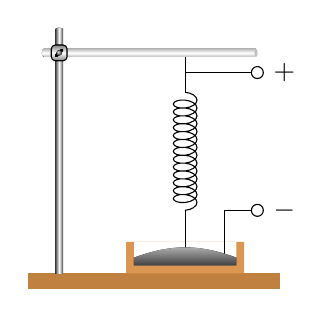
\begin{tikzpicture}[>=latex,scale=1.0]
  \fill[brown](-2,0)rectangle(1.2,0.2);
  \fill[brown7,even odd rule](-0.75,0.2)rectangle(0.75,0.6)(-0.65,0.3)rectangle(0.65,0.6);
  \draw[decorate,decoration={coil,segment length=1mm,amplitude=1.5mm}](0,2.5)--(0,1);
  \draw(0,1)--(0,0.5);
  \draw(0,3)--(0,2.5);
  \draw[-o](0.5,0.3)--(0.5,1)--(1,1)node[right]{$-$};
  \fill[top color=lightgray,bottom color=darkgray](-0.65,0.3)--(-0.65,0.4)to[bend left=20](0.65,0.4)--(0.65,0.3);
  \draw[-o](0,2.75)--(1,2.75)node[right]{$+$};
  \fill[left color=darkgray,right color=darkgray,middle color=white](-1.6,3.3)ellipse(0.05 and 0.02);
  \fill[left color=darkgray,right color=darkgray,middle color=white](-1.65,0.2)rectangle(-1.55,3.3);
  \fill[top color=lightgray,bottom color=lightgray,middle color=white](-1.8,3.0)ellipse(0.02 and 0.05);
  \fill[top color=lightgray,bottom color=lightgray,middle color=white](-1.8,2.95)rectangle(0.9,3.05);
  \fill[lightgray](0.9,3.0)ellipse(0.02 and 0.05);
  \fill[top color=gray,bottom color=gray,middle color=white,rounded corners=0.5mm,draw](-1.7,3.1)rectangle(-1.5,2.9);
  \draw[very thick,line cap=round]([shift=(-135:0.05)]-1.6,3.0)--++(45:0.1);
  \fill[ball color=gray](-1.6,3.0)circle(1pt);
\end{tikzpicture}
\end{document}